\setlength{\columnsep}{3pt}
\begin{flushleft}
	\textbf{Use case 1}
	\begin{itemize}
		\item Imagine there is a requirement to create 2 separate networks for \textbf{Finance} \& \textbf{HR department}.
		\item \textbf{Finance department} needs 50 IP address.
		\item \textbf{HR department} needs 30 IP address.
		\item Team manager have purchased a \textbf{network address - "16.0.0.0"}.
		\item \textbf{How would you use network address 16.0.0.0 and create 2 different network for finance \& HR department?}
		\begin{figure}[h!]
			\centering
			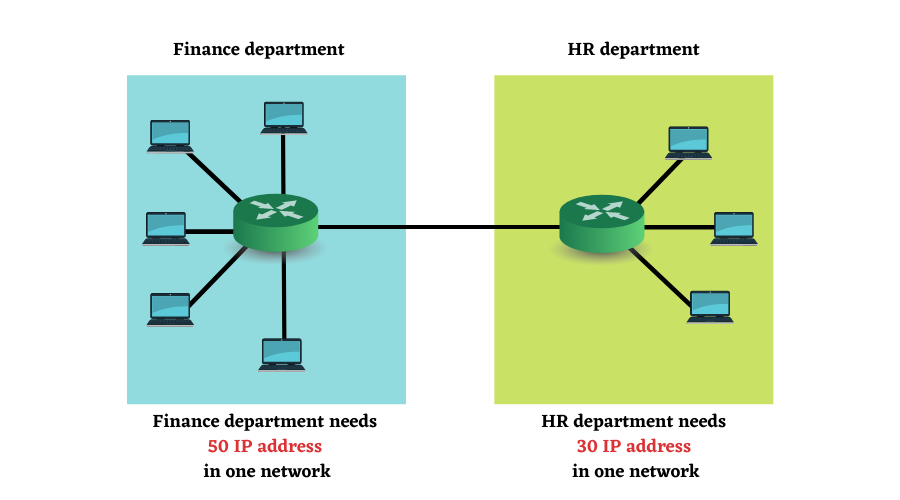
\includegraphics[scale=.65]{content/chapter14/images/depart.png}
			\caption{Custom IP address requirement}
			\label{fig:cidr}
		\end{figure}	
		\item Let's see how to do this.
	\end{itemize}
	
	\newpage
	\textbf{Solution}
	\newline
	Using Class A, B or C IP address range would result in lots of IP address wastage.
	\newline
	The solution is to logically divide the \textbf{16.0.0.0} network address into multiple different networks using CIDR.
	\newline
	Steps for CIDR:
	\begin{itemize}
		
		\item \textbf{Select a number "n"}:
		\begin{itemize}
			\item Decide maximum number of IP address you need in a single network. Here, \textbf{maximum number of IP needed is 50}.
			\item Select number "n" that can fit into below formula and is greater than or equal to 50.
			\bigskip
			\begin{tcolorbox}[breakable,notitle,boxrule=-0pt,colback=pink,colframe=pink]
				\color{black}
				Formula: $2^n-2 >= number\_of\_host\_ip\_needed$
				\fontdimen2\font=4pt
			\end{tcolorbox}
			\item Here, $2^n-2 >= 50$
			\item Solution: $2^6-2 >= 50$, where \textbf{n=6}
		\end{itemize}
		\item \textbf{Calculate new netmask:}
		\begin{itemize}
			\item To calculate new netmask:
			\bigskip
			\begin{tcolorbox}[breakable,notitle,boxrule=-0pt,colback=pink,colframe=pink]
				\color{black}
				Formula: 
				\newline
				OFF \textbf{n} bits from right to left
				\newline
				ON rest of the bits
				\fontdimen2\font=4pt
			\end{tcolorbox}
			\item Here n=6, so answer is:
			\begin{itemize}
				\item Binary form: \textbf{11111111.11111111.11111111.11000000}
				\item Netmask: \textbf{255.255.255.192}
				\item Netmask Prefix: \textbf{26}
			\end{itemize}
		\end{itemize}
		\item Total host IP in a network:
		\begin{itemize}
			\item Using value of \textbf{"n"}, total number of host IP are:
			\begin{tcolorbox}[breakable,notitle,boxrule=-0pt,colback=pink,colframe=pink]
				\color{black}
				Formula: $2^n-2$
				\fontdimen2\font=4pt
			\end{tcolorbox}
			\item Here, answer is: $2^6-2=62$
		\end{itemize}
		\newpage
		\item All networks possible for \textbf{16.0.0.0/26}:
		\begin{figure}[h!]
			\centering
			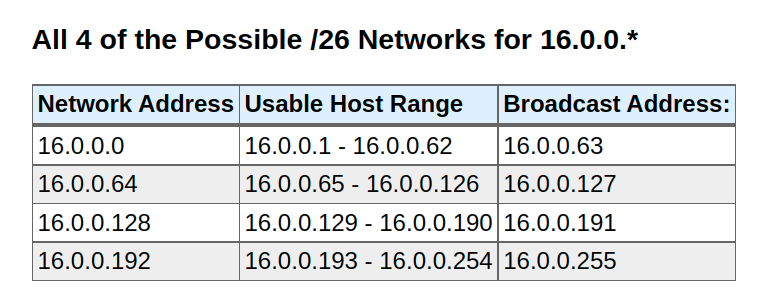
\includegraphics[scale=.4]{content/chapter14/images/possible.png}
			\caption{16.0.0.0/26 possible network address}
			\label{fig:cidr_new}
		\end{figure}	
		.
	\end{itemize}
.
\newpage
\newpage
\textbf{Use case 2}
\begin{itemize}
	\item Imagine there is a requirement to create 2 separate networks for \textbf{IT} \& \textbf{HR department}.
	\item \textbf{IT department} needs 24 IP address.
	\item \textbf{HR department} needs 10 IP address.
	\item Team manager have purchased an \textbf{IP address - "34.67.4.0"}.
	\item \textbf{How would you use IP address "34.67.4.0" and create 2 different network for IT \& HR department?}
	\begin{figure}[h!]
		\centering
		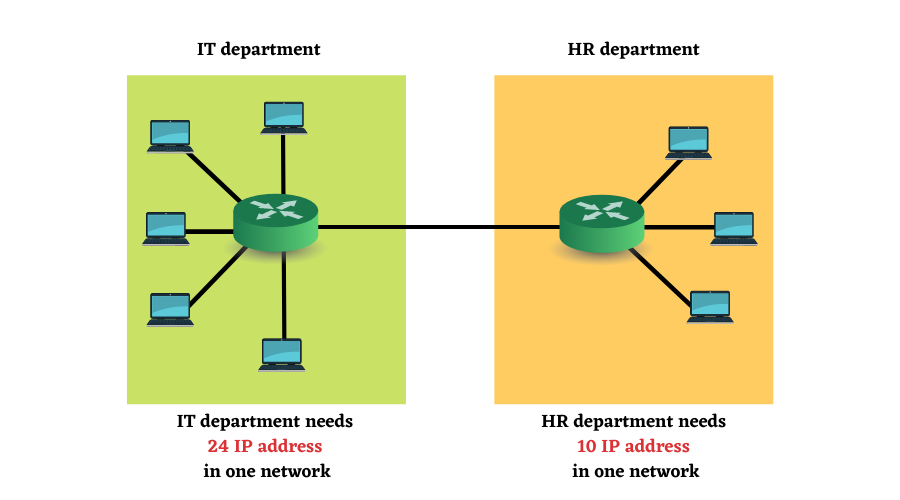
\includegraphics[scale=.65]{content/chapter14/images/depart3.png}
		\caption{Custom IP address requirement}
		\label{fig:cidr2}
	\end{figure}	
	\item Let's see how to do this.
\end{itemize}

\newpage
	\textbf{Solution}
\newline
Steps for CIDR:
\begin{itemize}
	
	\item \textbf{Select a number "n"}:
	\begin{itemize}
		\item Here, \textbf{maximum number of IP needed is 24}.
		\item Select number "n" that can fit into below formula and is greater than or equal to 24.
		\item Here, $2^n-2 >= 24$
		\item Solution: $2^5-2 >= 24$, where \textbf{n=5}
	\end{itemize}
	\item \textbf{Calculate new netmask:}
	\begin{itemize}
		\item Here n=5, so answer is:
		\begin{itemize}
			\item Binary form: \textbf{11111111.11111111.11111111.11100000}
			\item Netmask: \textbf{255.255.255.224}
			\item Netmask Prefix: \textbf{27}
		\end{itemize}
	\end{itemize}
	\item Total host IP in a network:
	\begin{itemize}
		\item Using value of \textbf{"n"}, total number of host IP are:
		\begin{tcolorbox}[breakable,notitle,boxrule=-0pt,colback=pink,colframe=pink]
			\color{black}
			Formula: $2^n-2$
			\fontdimen2\font=4pt
		\end{tcolorbox}
		\item Here, answer is: $2^5-2=30$
	\end{itemize}
	\item All networks possible for \textbf{34.67.4.0/27}:
	\begin{figure}[h!]
		\centering
		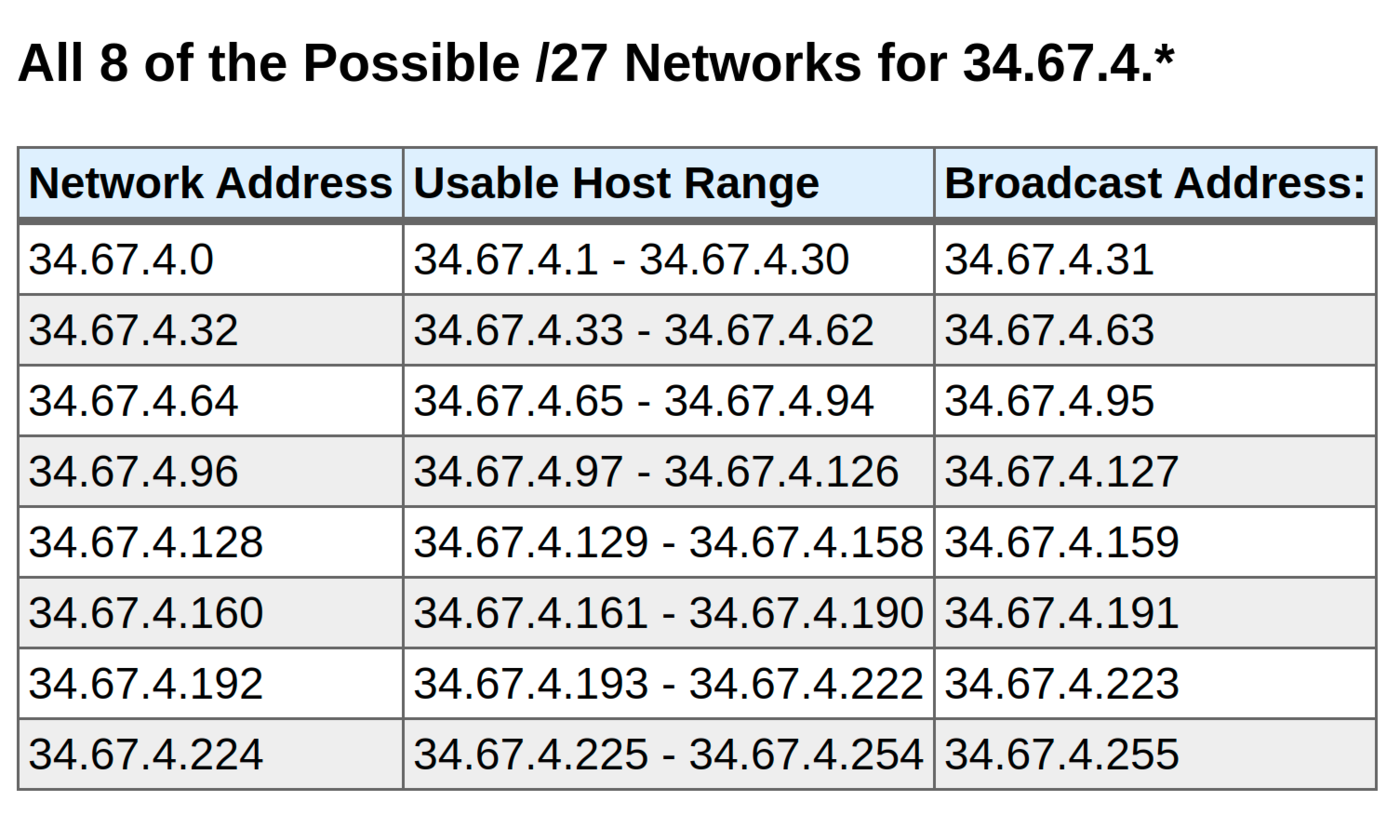
\includegraphics[scale=.2]{content/chapter14/images/possible2.png}
		\caption{34.67.4.0/27 possible network address}
		\label{fig:cidr_new_2}
	\end{figure}	
	.
\end{itemize}
.
\newpage
\newpage	
	
\end{flushleft}
\newpage


